%package list
\documentclass{article}
\usepackage[top=3cm, bottom=3cm, outer=3cm, inner=3cm]{geometry}
\usepackage{multicol}
\usepackage{graphicx}
\usepackage{url}
%\usepackage{cite}
\usepackage{hyperref}
\usepackage{array}
%\usepackage{multicol}
\newcolumntype{x}[1]{>{\centering\arraybackslash\hspace{0pt}}p{#1}}
\usepackage{natbib}
\usepackage{pdfpages}
\usepackage{multirow}
\usepackage[normalem]{ulem}
\useunder{\uline}{\ul}{}
\usepackage{svg}
\usepackage{xcolor}
\usepackage{listings}
\lstdefinestyle{ascii-tree}{
    literate={├}{|}1 {─}{--}1 {└}{+}1 
  }
\lstset{basicstyle=\ttfamily,
  showstringspaces=false,
  commentstyle=\color{red},
  keywordstyle=\color{blue}
}
%\usepackage{booktabs}
\usepackage{caption}
\usepackage{subcaption}
\usepackage{float}
\usepackage{array}

\newcolumntype{M}[1]{>{\centering\arraybackslash}m{#1}}
\newcolumntype{N}{@{}m{0pt}@{}}


%%%%%%%%%%%%%%%%%%%%%%%%%%%%%%%%%%%%%%%%%%%%%%%%%%%%%%%%%%%%%%%%%%%%%%%%%%%%
%%%%%%%%%%%%%%%%%%%%%%%%%%%%%%%%%%%%%%%%%%%%%%%%%%%%%%%%%%%%%%%%%%%%%%%%%%%%
\newcommand{\itemEmail}{}
\newcommand{\itemStudent}{Arce Mayhua Leonardo  Velasque Arcos Mikhail  Quispe Saavedra Dennis Choquehuanca Bedoya Brayan }
\newcommand{\itemCourse}{Programación web 2}
\newcommand{\itemCourseCode}{}
\newcommand{\itemSemester}{I}
\newcommand{\itemUniversity}{Universidad Nacional de San Agustín de Arequipa}
\newcommand{\itemFaculty}{Facultad de Ingeniería de Producción y Servicios}
\newcommand{\itemDepartment}{Departamento Académico de Ingeniería de Sistemas e Informática}
\newcommand{\itemSchool}{Escuela Profesional de Ingeniería de Sistemas}
\newcommand{\itemAcademic}{2024 - A}
\newcommand{\itemInput}{Del 26 Mayo 2024}
\newcommand{\itemOutput}{Al 2 Junio  2024}
\newcommand{\itemPracticeNumber}{05}
\newcommand{\itemTheme}{Python}
%%%%%%%%%%%%%%%%%%%%%%%%%%%%%%%%%%%%%%%%%%%%%%%%%%%%%%%%%%%%%%%%%%%%%%%%%%%%
%%%%%%%%%%%%%%%%%%%%%%%%%%%%%%%%%%%%%%%%%%%%%%%%%%%%%%%%%%%%%%%%%%%%%%%%%%%%

\usepackage[english,spanish]{babel}
\usepackage[utf8]{inputenc}
\AtBeginDocument{\selectlanguage{spanish}}
\renewcommand{\figurename}{Figura}
\renewcommand{\refname}{Referencias}
\renewcommand{\tablename}{Tabla} %esto no funciona cuando se usa babel
\AtBeginDocument{%
	\renewcommand\tablename{Tabla}
}

\usepackage{fancyhdr}
\pagestyle{fancy}
\fancyhf{}
\setlength{\headheight}{30pt}
\renewcommand{\headrulewidth}{1pt}
\renewcommand{\footrulewidth}{1pt}
\fancyhead[L]{\raisebox{-0.2\height}{
\includegraphics[width=3cm]{img/logo_episunsa.png}}}
\fancyhead[C]{\fontsize{7}{7}\selectfont	\itemUniversity \\ \itemFaculty \\ \itemDepartment \\ \itemSchool \\ \textbf{\itemCourse}}
\fancyhead[R]{\raisebox{-0.2\height}{
\includegraphics[width=1.2cm]{img/logo_abet}}}
\fancyfoot[L]{Integrantes}
\fancyfoot[C]{\itemCourse}
\fancyfoot[R]{Página \thepage}

% para el codigo fuente
\usepackage{listings}
\usepackage{color, colortbl}
\definecolor{dkgreen}{rgb}{0,0.6,0}
\definecolor{gray}{rgb}{0.5,0.5,0.5}
\definecolor{mauve}{rgb}{0.58,0,0.82}
\definecolor{codebackground}{rgb}{0.95, 0.95, 0.92}
\definecolor{tablebackground}{rgb}{0.8, 0, 0}

\lstset{frame=tb,
	language=bash,
	aboveskip=3mm,
	belowskip=3mm,
	showstringspaces=false,
	columns=flexible,
	basicstyle={\small\ttfamily},
	numbers=none,
	numberstyle=\tiny\color{gray},
	keywordstyle=\color{blue},
	commentstyle=\color{dkgreen},
	stringstyle=\color{mauve},
	breaklines=true,
	breakatwhitespace=true,
	tabsize=3,
	backgroundcolor= \color{codebackground},
}

\begin{document}
	
	\vspace*{10px}
	
	\begin{center}	
		\fontsize{17}{17} \textbf{ Informe de Laboratorio \itemPracticeNumber}
	\end{center}
	\centerline{\textbf{\Large Tema: \itemTheme}}
	%\vspace*{0.5cm}	

	\begin{flushright}
		\begin{tabular}{|M{2.5cm}|N|}
			\hline 
			\rowcolor{tablebackground}
			\color{white} \textbf{Nota}  \\
			\hline 
			     \\[30pt]
			\hline 			
		\end{tabular}
	\end{flushright}	

	\begin{table}[H]
		\begin{tabular}{|x{4.7cm}|x{4.8cm}|x{4.8cm}|}
			\hline 
			\rowcolor{tablebackground}
			\color{white} \textbf{Estudiante} & \color{white}\textbf{Escuela}  & \color{white}\textbf{Asignatura}   \\
			\hline 
			{\itemStudent \par \itemEmail} & \itemSchool & {\itemCourse \par Semestre: \itemSemester \par Código: \itemCourseCode}     \\
			\hline 			
		\end{tabular}
	\end{table}		
	
	\begin{table}[H]
		\begin{tabular}{|x{4.7cm}|x{4.8cm}|x{4.8cm}|}
			\hline 
			\rowcolor{tablebackground}
			\color{white}\textbf{Laboratorio} & \color{white}\textbf{Tema}  & \color{white}\textbf{Duración}   \\
			\hline 
			\itemPracticeNumber & \itemTheme & 04 horas   \\
			\hline 
		\end{tabular}
	\end{table}
	
	\begin{table}[H]
		\begin{tabular}{|x{4.7cm}|x{4.8cm}|x{4.8cm}|}
			\hline 
			\rowcolor{tablebackground}
			\color{white}\textbf{Semestre académico} & \color{white}\textbf{Fecha de inicio}  & \color{white}\textbf{Fecha de entrega}   \\
			\hline 
			\itemAcademic & \itemInput &  \itemOutput  \\
			\hline 
		\end{tabular}
	\end{table}
	\section{INTRODUCCION}
	\begin{itemize}		
		\item En el siguiente informe expondre las actividades del laboratorio 05 del curso de programacion web 02 ,
		\item La exposcion de los ejercicios seran de la siguiente manera
		\item Primero:Expondre las partes mas importantes del codigo, en este caso los metodos ,centrandonos en la logica de estos
		\item Segundo:Expondremos los ejercicios explicando el uso de los metodos para la resolucion de los ejercicios
	\end{itemize}
	\section{Clase Picture }
	\begin{itemize}		
		\item Los metodos desarrollados por el equipo estaran en la clase picture 
		\item verticalMirror()
		\item Devuelve el espejo vertical de la imagen
		\begin{lstlisting}[language=Python, caption={VerticalMirror}, float=H]
			def verticalMirror(self):
    vertical = []
    for value in self.img:
      vertical.append(value[::-1])

    return Picture(vertical)
        \end{lstlisting}
		\item En este metodo iteraremos sobre la imagen dada como atributo 
		\item Crearemos una imagen vacia(lista) y le daremos los valores de la imagen entregada,pero de manera inversa 
		      para esto utilizaremos  la expresion slice en cada string de la imagen , -1 indicara que comenzara desde el ultimo elemento y el primer: indicara al siguiente 
			  de esta manera se invertiran todos los caracteres del string para su posterior agregacion a nueva imagen.
		\item Este metodo lo usaremos en el ejercicio 2b
		
		\item horizontalMirror()
		\item Devuelve el espejo horizontal de la imagen
		\begin{lstlisting}[language=Python, caption={horizontalMirror}, float=H]
			def horizontalMirror(self):
    horizontal = []
    for value in reversed(self.img):
      horizontal.append(value)
    return Picture(horizontal)
        \end{lstlisting}
		\item En este metodo iteraremos sobre la imagen dada como atributo 
		\item Crearemos una imagen vacia(lista) y le daremos los valores de la imagen entregada,pero de manera invertida  
		      para iteraremos con el metodo reversed lo que nos dara el ultimo elemento al primero , lo que permitira que la imagen se muestre de cabeza
			   devido a que la nueva imagen tendra como primer elemento el ultimo string de la imagen original y asi hasta el primer elemento de la imagen original 
		\item Este metodo quedara obsoleto 

	\item negative()
		\item Devuelve el negativo de la imagen
		\begin{lstlisting}[language=Python, caption={negative}, float=H]
			def negative(self):
    nuevaImagen = []
    for value in self.img:
      row = []
      for caracter in value:
        row.append(self._invColor(caracter))
      nuevaImagen.append(row)    
    return Picture(nuevaImagen)
        \end{lstlisting}
		\item En este metodo cambiaremos el color de la imagen dada con su inverso
		\item Crearemos una imagen vacia(lista) , luego iteraremos sobre la imagen y agregaremos a la nueva imagen los strings invertidos de la 
		      imagen original , esto sera posible gracias a el motodo _invColor que usa el diccionario inverter de la calse Color , este diccionario tiene como
			  llave un elemento que puede cambiar de color , solo seran 4 los elementos que tendran inversa _invColor retornara el inverso del caracter y lo agregara a la nueva imagen
			  de esta manera se obtendra el inverso de cada pieza del ajedrez 
		\item Este metodo se utilizara mucho en varios ejercicio destacando su uso en el ejericicio 2g.
		
		\item join()
		\item pone la imagen al lado derecho usando el argumento p
		\begin{lstlisting}[language=Python, caption={Join}, float=H]
			def join(self, p):
    nuevaImagen = []

    for index, value in enumerate(self.img):
      nuevaImagen.append(list(value) + list(p.img[index]))

    return Picture(nuevaImagen)
        \end{lstlisting}
		\item En este metodo crearemos una imagen que tendra a su costado otra imagen ,algo parecido a una concatenacion
		\item Crearemos una imagen vacia, iteraremos sobre la imagen dada ,en este caso nos pasaran dos imagenes pero como el taño es el mismo solo usaremos index como indice de la segunda imagen
		      luego simplemente concatenaremos los strings de las dos imagenes brindadas osea , el primer string de la primera imagen se concatenara con el primer string de la segunda imagen ,su concatenacion sera 
			  agregada al primer elemento de la nueva imagen y asi con todos los elementos, deesta manera se podra colocar una imagen al costado de otra.  
     	\item Este metodo se utilizara en algunos otros metodos como horizontalRepeat.
     	
		 \item up()
		 \item Devuelve a la figura encima de la actual
		 \begin{lstlisting}[language=Python, caption={up}, float=H]
			def up(self, p):
			nuevaImagen = []
			#copiar todo p a nueva imange
			for value in p.img:
			  nuevaImagen.append(value)
			
			for value in self.img:
			  nuevaImagen.append(value)
			return Picture(nuevaImagen)		
		 \end{lstlisting}
		 \item En este metodo crearemos una imagen que tendra encima a otra imagen 
		 \item Crearemos una imagen vacia, iteraremos respectivamente con las imagenes dadas, en la iteracion de la primera imagen 
		       agregaremos los elemento a la imagen vacia creada ,luego iteraremos sobre la segunda imagen y seguiremos añadiendo estos elementos a la imagen anteriormente vacia
			   lo que tendremos sera una imagen con el doble de longitud de una imagen normal lo que dara la impresion de que una pieza esta encima de la otra  
		 \item Este metodo se utilizara en algunos otros metodos como verticalRepeat.
		 
		 \item under()
		 \item Devuelve una nueva imagen  y la sobrepone encima de la actual
		 \begin{lstlisting}[language=Python, caption={under}, float=H]
			def under(self, p):
    nuevaImagen = []
    for value in self.img:
        nuevaImagen.append(list(value))

    for i, value in enumerate(p.img):
      for j, caracter in enumerate(value):
        if(nuevaImagen[i][j] == ' '):
          nuevaImagen[i][j] = caracter

    return Picture(nuevaImagen)	
		 \end{lstlisting}
		 \item En este metodo crearemos una imagen que sobrepondra otra imagen dando una simulacion como un cudrado del ajedres con su pieza encima
		 \item Crearemos una imagen vacia , e iteraremos sobre la imagen que tiene la figura de una pieza, luego haremos una iteracion anidad para consultar todos los caracteres de la nueva imagen
		        dentro del bucle anidado utilizaremos una condicional para saber que caracteres de la nueva iamgen se encuentran vacios (" ") ,y caso que este vacio colocaremos el caracter de la otra imagen que sera 
				un square de esta manera se colocara la pieza encima de su cuadrado de ajedres
		 \item Este metodo se utilizara en el ultimo ejercicio 2g.
		 
		 \item horizontalRepeat()
		 \item Devuelve una nueva figura repitiendo la figura actual al costado
		 la cantidad de veces que indique el valor de n
		 \begin{lstlisting}[language=Python, caption={horizontalRepeat}, float=H]
			def horizontalRepeat(self, n):
			aux = self
			for _ in range(n-1):
			  aux = aux.join(self) 
			return aux
		 \end{lstlisting}
		 \item En este metodo crearemos una imagen que tendra n veces a la misma imagen a su lado
		 \item Crearemos una imagen qeu tendra lo mismo que la imagen principal sobre todo para que nuestra imagen original no quede modificada , luego iteraremos n-1 veces debido
		       a que utilizaremos el metodo join dentro de este bucle , por lo que el trabajo de duplicar n veces la imagen lo hara join ,sin embargo como en la primera iteracion genera2 imagenes se tendra qeu iterar n-1 veces
			   , de esta manera colocaremos n veces la imagen al cosatado de la misma imagen   
		 \item Este metodo se utilizara en el ejercicio 2c.
		 
		 \item verticalRepeat()
		 \item Devuelve una nueva figura repitiendo la figura actual debajo, la cantidad
		 de veces que indique el valor de n
		 \begin{lstlisting}[language=Python, caption={verticalRepeat}, float=H]
			def verticalRepeat(self, n):
			aux = self
			for _ in range(n-1):
			  aux = aux.up(self) 
			return aux
		 \end{lstlisting}
		 \item En este metodo crearemos una imagen que tendra n veces a la misma imagen encima
		 \item Este metodo se comportara de la misma manera que en anterior metodo , con la diferencia que dentro de las iteraciones se llamara al metodo up envez del join
		       lo que permitira sobre poner n veces la imagen .
		 \item Este metodo se utilizara en varios ejercicios.
	\end{itemize} 
	
	\section{Código del ejercicio 2a}
	\begin{itemize}
        \begin{lstlisting}[language=Python, caption={Código del ejercicio A}]
            from chessPictures import *
            from interpreter import draw

            tab = knight
            # Une el caballo con su inverso
            tab = Picture.join(tab, Picture.negative(knight)) 
         \end{lstlisting}

        \item Tablero resultante del ejercicio A
         \begin{lstlisting}[language=Python, caption={Tablero resultante del ejercicio A}]
         # Muestra el tablero resultante
        draw(Picture.up(Picture.negative(tab), tab))
         \end{lstlisting}
		 \begin{figure}[H]
			\centering
			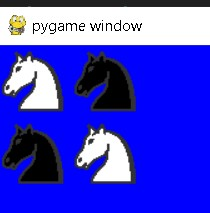
\includegraphics[scale=0.3]{img/ejercicio2a.jpg}
		\end{figure}
	\end{itemize} 
        \section{Código del ejercicio B}
		\begin{itemize}
        \begin{lstlisting}[language=Python, caption={Código del ejercicio B}]
        from chessPictures import *
        from interpreter import draw

        tab = knight
       # Une el caballo con su inverso
        tab = Picture.join(tab, Picture.negative(knight))
       # Refleja verticalmente y muestra el tablero resultante
       tab = Picture.up(Picture.verticalMirror(tab), tab)
       \end{lstlisting}
       \item Tablero resultante del ejercicio B
        \begin{lstlisting}[language=Python, caption={Tablero resultante del ejercicio B}]
        # Muestra el tablero resultante
        draw(tab)
        \end{lstlisting}
		\begin{figure}[H]
			\centering
			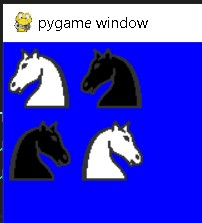
\includegraphics[scale=0.3]{img/ejercicio2b.jpg}
		\end{figure}
	\end{itemize} 
        \section{Código del ejercicio C}
		\begin{itemize}
        \begin{lstlisting}[language=Python, caption={Código del ejercicio C}]
         from interpreter import draw
         from chessPictures import *

         # Repite horizontalmente la imagen del rey cuatro veces
         draw(king.horizontalRepeat(4))
         \end{lstlisting}
		 \begin{figure}[H]
			\centering
			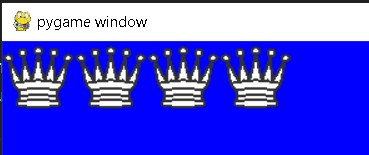
\includegraphics[scale=0.3]{img/ejercicio2c.jpg}
		\end{figure}
	\end{itemize} 
	\section{Ejercicio2d}
\begin{itemize}   
    \item Creación del cuadro inicial del tablero
    \begin{lstlisting}[language=Python, caption={Creacion de un primer cuadro}, float=H]
	eb = Picture(SQUARE)
    \end{lstlisting}
    \item Creación del cuadro de color negativo(color negro)
    \begin{lstlisting}[language=Python, caption={Creacion de un primer cuadro negativo}, float=H]
	en = eb.negative()
    \end{lstlisting}
    \item Se concluye el ejercicio imprimiendo la imagen fusionada de el cuadro normal y su negativo al costado, a esta imagen se le repite con "horizontalRepeat" 4 veces.
    \begin{lstlisting}[language=Python, caption={Creacion e impresion de una fila}, float=H]
	draw(eb.join(en).horizontalRepeat(4))
    \end{lstlisting}
    \item Ver impresión:
    \begin{figure}[H]
		\centering
		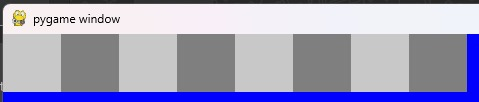
\includegraphics[scale=0.3]{img/ejercicio2d.jpg}
	\end{figure}
\end{itemize}

\section{Ejercicio2e}
\begin{itemize}   
    \item Se realiza lo mismo que el ejercicio anterior pero el orden de invocación de los cuadros se invierte en este caso primero se pone el negativo "en".
    \begin{lstlisting}[language=Python, caption={Creacion e impresion de una fila con primer cuadro negativo}, float=H]
	draw(en.join(eb).horizontalRepeat(4))
    \end{lstlisting}
    \item Ver impresión:
    \begin{figure}[H]
		\centering
		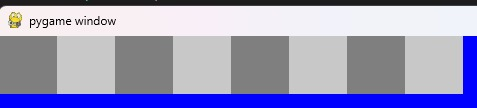
\includegraphics[scale=0.3]{img/ejercicio2e.jpg}
	\end{figure}
\end{itemize}

\section{Ejercicio2f}
\begin{itemize}   
    \item En este caso reutilizaremos las iniciaciones de los cuadros de los ejercicios anteriores.
	
    \begin{lstlisting}[language=Python, caption={Creacion e impresion de medio tablero}, float=H]
	eb = Picture(SQUARE)
	en = eb.negative()
	fila1 = eb.join(en).horizontalRepeat(4)
	fila2 = en.join(eb).horizontalRepeat(4)
	imagen = fila2.up(fila1).verticalRepeat(2)
	draw(imagen)
    \end{lstlisting}
    en "imagen" se junta de manera horizontal la fila2 a la fila1 y se hace vertical repeat 2 veces lo que nos retorna un tablero de 4X8.
    \item Ver impresión:
	\begin{figure}[H]
		\centering
		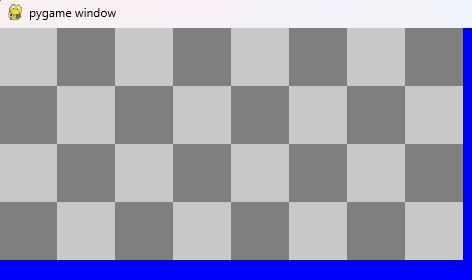
\includegraphics[scale=0.3]{img/ejercicio2f.jpg}
	\end{figure}
\end{itemize}
	\section{Clase o tablero del Ajedrez(Ejercicio 2g)}
    \begin{itemize}
        \item En esta sección se utilizarán métodos avanzados de manipulación de imágenes desarrollados hasta ahora, como el método de inversión, que toma la imagen y la invierte, y el método de repetición, que toma la imagen y la repite de forma horizontal o vertical.
        \item Creación de la fila inicial para las piezas blancas:
         \begin{lstlisting}[language=Python, caption={Fila inicial para piezas blancas}, float=H]
from chessPictures import *
from interpreter import draw
from picture import Picture
from colors import *

filaInicial = Picture.under(rock, Picture.negative(square))
filaInicial = Picture.join(filaInicial, Picture.under(knight, square))
filaInicial = Picture.join(filaInicial, Picture.under(bishop, Picture.negative(square)))
filaInicial = Picture.join(filaInicial, Picture.under(queen, square))
filaInicial = Picture.join(filaInicial, Picture.under(king, Picture.negative(square)))
filaInicial = Picture.join(filaInicial, Picture.under(bishop, square))
filaInicial = Picture.join(filaInicial, Picture.under(knight, Picture.negative(square)))
filaInicial = Picture.join(filaInicial, Picture.under(rock, square))
         \end{lstlisting}
    \item Se crea una fila con las piezas blancas en su posición inicial alternando los colores de los cuadrados.
    \item Creación de la fila inicial para las piezas negras:
    \begin{lstlisting}[language=Python, caption={Fila inicial para piezas negras}, float=H]
                    filaNegro = Picture.negative(filaInicial)
    \end{lstlisting}
    \item Se invierten los colores de la fila inicial blanca para obtener la fila inicial negra.
    \item Creación de la fila de peones:
    \begin{lstlisting}[language=Python, caption={Fila de peones}, float=H]
filaPeon = Picture.under(pawn, square)
filaPeon = Picture.join(filaPeon, Picture.under(pawn, Picture.negative(square)))
filaPeon = Picture.horizontalRepeat(filaPeon, 4)
    \end{lstlisting}
    \item Se crea una fila de peones alternando colores y repitiendo el patrón para obtener 8 peones.
    \item Creación de un patrón de tablero de ajedrez vacío:
    \begin{lstlisting}[language=Python, caption={Patrón de tablero vacío}, float=H]
tabla1 = square
tabla1 = Picture.join(tabla1, Picture.negative(square))
tabla1 = (Picture.horizontalRepeat(tabla1, 4))
tabla2 = Picture.negative(tabla1)
tabla3 = Picture.verticalRepeat(Picture.up(tabla2, tabla1), 2)
    \end{lstlisting}
    \item Se crea un patrón de tablero vacío de 8x8 cuadrados alternando los colores.
    \item Construcción del tablero completo con piezas:
    \begin{lstlisting}[language=Python, caption={Tablero completo con piezas}, float=H]
tablero = Picture.up(Picture.negative(filaPeon), filaNegro)
tablero = Picture.up(tabla3, tablero)
tablero = Picture.up(filaPeon, tablero)
tablero = Picture.up(filaInicial, tablero)

draw(tablero)
    \end{lstlisting}
    \item Se colocan las filas de piezas y peones en el tablero vacío para formar el tablero completo.
    \item Ver la creación de la imagen:
	\begin{figure}[H]
		\centering
		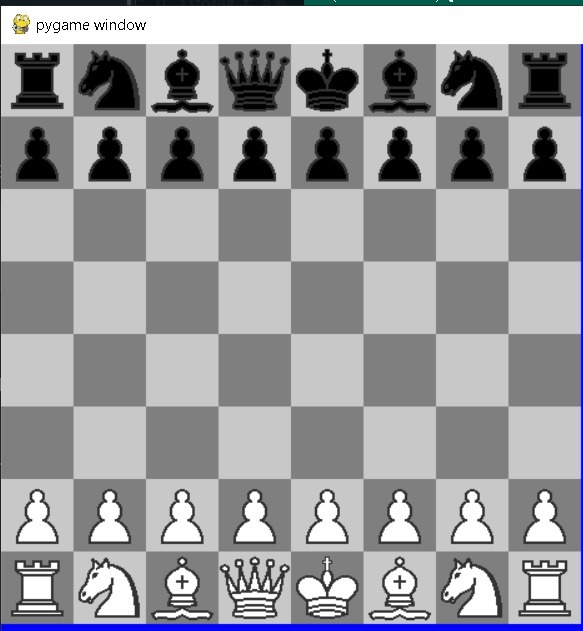
\includegraphics[scale=0.3]{img/tablerro_Ajedres.jpg}
	\end{figure}
    \item Código completo:
    \begin{lstlisting}[language=Python, caption={Código completo}, float=H]
from chessPictures import *
from interpreter import draw
from picture import Picture
from colors import *

#Ejercicio g tablero completo

filaInicial = Picture.under(rock, Picture.negative(square))
filaInicial = Picture.join(filaInicial, Picture.under(knight, square))
filaInicial = Picture.join(filaInicial, Picture.under(bishop, Picture.negative(square)))
filaInicial = Picture.join(filaInicial, Picture.under(queen, square))
filaInicial = Picture.join(filaInicial, Picture.under(king, Picture.negative(square)))
filaInicial = Picture.join(filaInicial, Picture.under(bishop, square))
filaInicial = Picture.join(filaInicial, Picture.under(knight, Picture.negative(square)))
filaInicial = Picture.join(filaInicial, Picture.under(rock, square))

filaNegro = Picture.negative(filaInicial)

filaPeon = Picture.under(pawn, square)
filaPeon = Picture.join(filaPeon, Picture.under(pawn, Picture.negative(square)))
filaPeon = Picture.horizontalRepeat(filaPeon, 4)

tabla1 = square
tabla1 = Picture.join(tabla1, Picture.negative(square))
tabla1 = (Picture.horizontalRepeat(tabla1, 4))
tabla2 = Picture.negative(tabla1)
tabla3 = Picture.verticalRepeat(Picture.up(tabla2, tabla1), 2)

tablero = Picture.up(Picture.negative(filaPeon), filaNegro)
tablero = Picture.up(tabla3, tablero)
tablero = Picture.up(filaPeon, tablero)
tablero = Picture.up(filaInicial, tablero)

draw(tablero)
    \end{lstlisting}
\end{itemize}
	\section{URL GitHub }
	\begin{itemize}
		\item \url{https://github.com/mvelasquea/Pweb2_E_04.git}
	\end{itemize}
	\section{Commits }
	\begin{itemize}
		\begin{figure}[H]
			\centering
			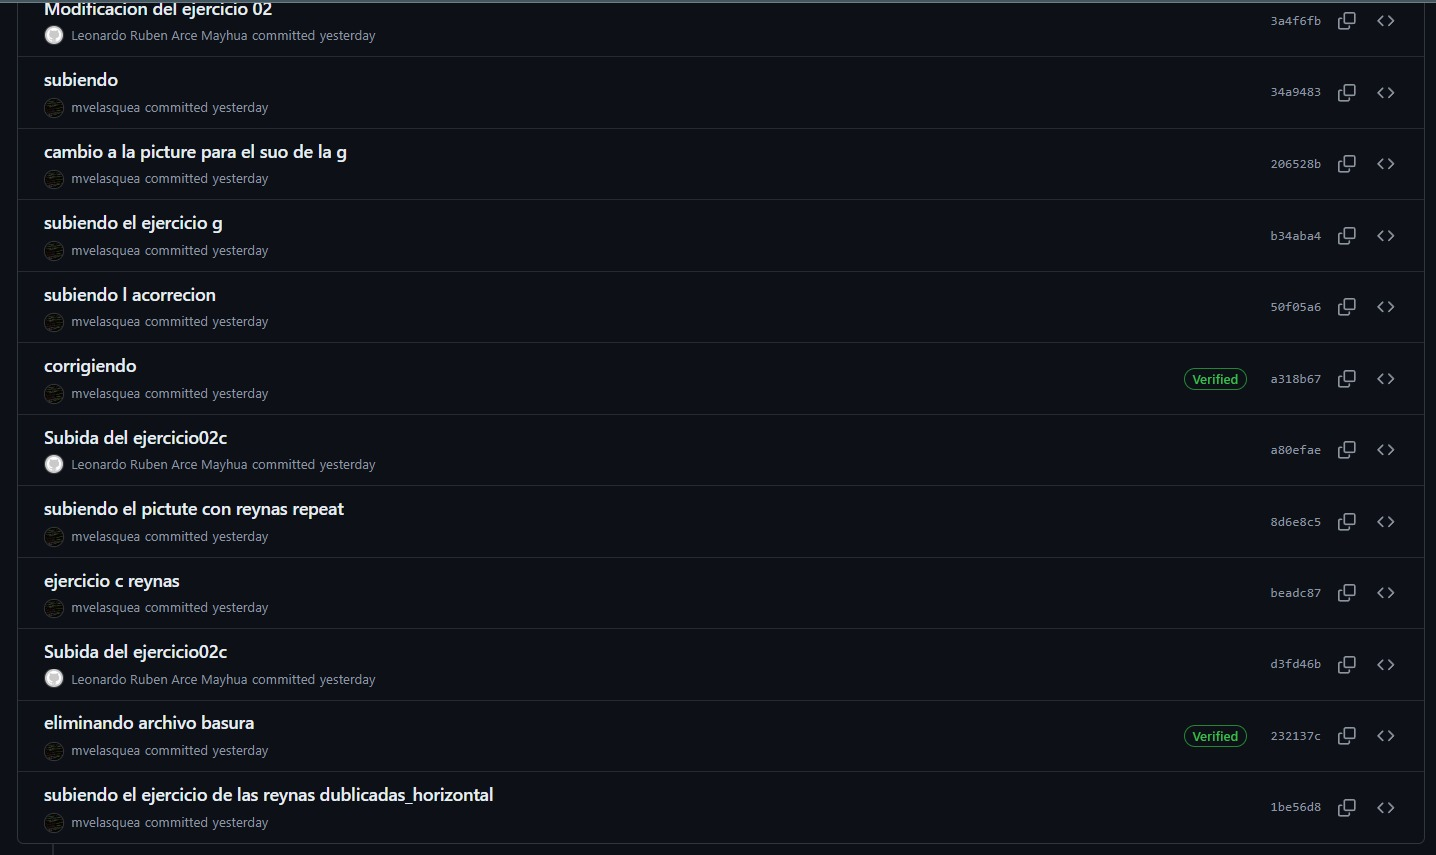
\includegraphics[scale=0.3]{img/commits1.jpg}
		\end{figure}
		\begin{figure}[H]
			\centering
			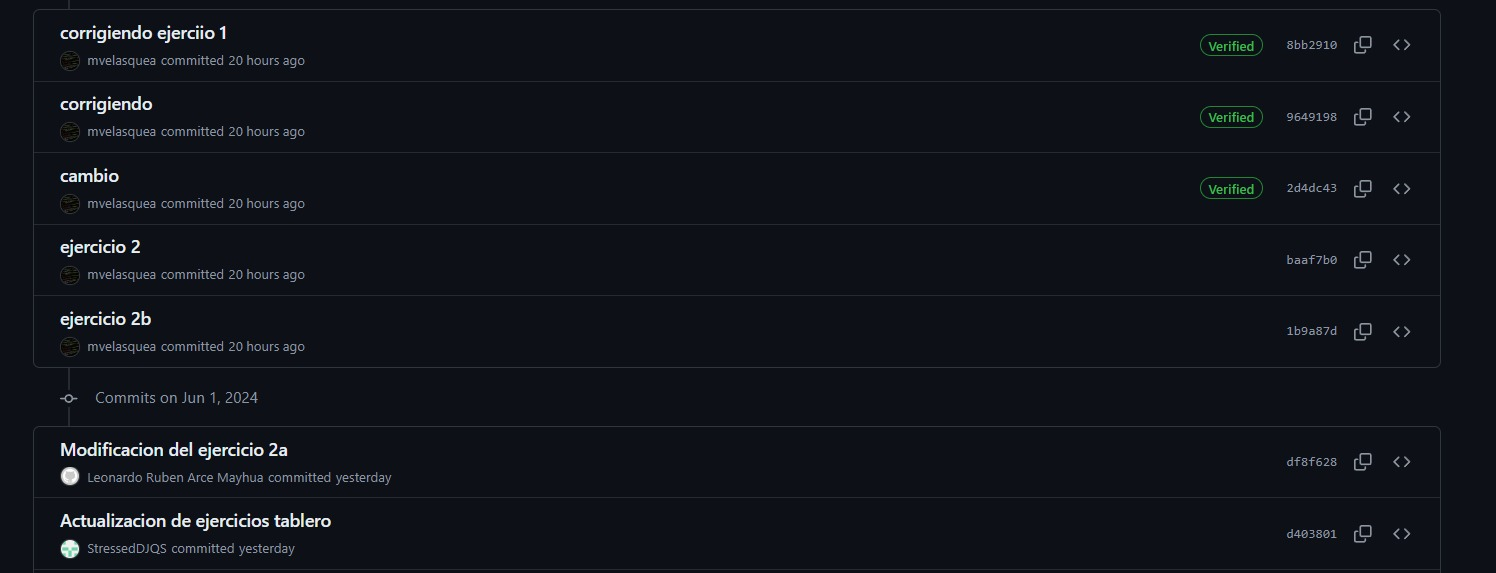
\includegraphics[scale=0.3]{img/commits2.jpg}
		\end{figure}
	\end{itemize}
	\section{\textcolor{red}{Rúbricas}}
	
\subsection{\textcolor{red}{Rúbrica para entregable Informe}}

\begin{table}[H]
    \caption{Rúbrica para tipo de Informe}
    \setlength{\tabcolsep}{0.5em} % for the horizontal padding
    {\renewcommand{\arraystretch}{1.5}% for the vertical padding
    \begin{tabular}{|p{3cm}|p{10cm}|p{2cm}|p{2cm}|}
        \hline
        \multicolumn{2}{|c|}{\textbf{Informe}} & \textbf{Cumple} & \textbf{No cumple} \\
        \hline
        \textbf{Latex} & El informe está en formato PDF desde Latex, con un formato limpio (buena presentación) y fácil de leer. & 20 & 17 \\ 
        \hline
        \textbf{MarkDown} & El informe está en formato PDF desde MarkDown README.md, con un formato limpio (buena presentación) y fácil de leer. & 17 & 0 \\ 
        \hline
        \textbf{MS Word} & El informe está en formato PDF desde plantilla MS Word, con un formato limpio (buena presentación) y fácil de leer. & 15 & 0 \\ 
        \hline
        \textbf{Observaciones} & Por cada observación se le descontará puntos. & - & - \\
        \hline
    \end{tabular}
    }
\end{table}
	\subsection{\textcolor{red}{Rúbrica para el contenido del Informe y demostración}}
	\begin{itemize}			
		\item El alumno debe marcar o dejar en blanco en celdas de la columna \textbf{Checklist} si cumplio con el ítem correspondiente.
		\item Si un alumno supera la fecha de entrega,  su calificación será sobre la nota mínima aprobada, siempre y cuando cumpla con todos lo items.
		\item El alumno debe autocalificarse en la columna \textbf{Estudiante} de acuerdo a la siguiente tabla:
	
		\begin{table}[ht]
			\caption{Niveles de desempeño}
			\begin{center}
			\begin{tabular}{ccccc}
    			\hline
    			 & \multicolumn{4}{c}{Nivel}\\
    			\cline{1-5}
    			\textbf{Puntos} & Insatisfactorio 25\%& En Proceso 50\% & Satisfactorio 75\% & Sobresaliente 100\%\\
    			\textbf{2.0}&0.5&1.0&1.5&2.0\\
    			\textbf{4.0}&1.0&2.0&3.0&4.0\\
    		\hline
			\end{tabular}
		\end{center}
	\end{table}	
	
	\end{itemize}
	
	\begin{table}[H]
		\caption{Rúbrica para contenido del Informe y demostración}
		\setlength{\tabcolsep}{0.5em} % for the horizontal padding
		{\renewcommand{\arraystretch}{1.5}% for the vertical padding
		%\begin{center}
		\begin{tabular}{|p{2.7cm}|p{7cm}|x{1.3cm}|p{1.2cm}|p{1.5cm}|p{1.1cm}|}
			\hline
    		\multicolumn{2}{|c|}{Contenido y demostración} & Puntos & Checklist & Estudiante & Profesor\\
			\hline
			\textbf{1. GitHub} & Hay enlace URL activo del directorio para el  laboratorio hacia su repositorio GitHub con código fuente terminado y fácil de revisar. &2 &X &1 & \\ 
			\hline
			\textbf{2. Commits} &  Hay capturas de pantalla de los commits más importantes con sus explicaciones detalladas. (El profesor puede preguntar para refrendar calificación). &4 &X &2 & \\ 
			\hline 
			\textbf{3. Código fuente} &  Hay porciones de código fuente importantes con numeración y explicaciones detalladas de sus funciones. &2 &X &2 & \\ 
			\hline 
			\textbf{4. Ejecución} & Se incluyen ejecuciones/pruebas del código fuente  explicadas gradualmente. &2 &X &2 & \\ 
			\hline			
			\textbf{5. Pregunta} & Se responde con completitud a la pregunta formulada en la tarea.  (El profesor puede preguntar para refrendar calificación).  &2 &X &2 & \\ 
			\hline	
			\textbf{6. Fechas} & Las fechas de modificación del código fuente estan dentro de los plazos de fecha de entrega establecidos. &2 &X &2 & \\ 
			\hline 
			\textbf{7. Ortografía} & El documento no muestra errores ortográficos. &2 &X &1 & \\ 
			\hline 
			\textbf{8. Madurez} & El Informe muestra de manera general una evolución de la madurez del código fuente,  explicaciones puntuales pero precisas y un acabado impecable.   (El profesor puede preguntar para refrendar calificación).  &4 &X &3 & \\ 
			\hline
			\multicolumn{2}{|c|}{\textbf{Total}} &20 & &16 & \\ 
			\hline
		\end{tabular}
		%\end{center}
		%\label{tab:multicol}
		}
	\end{table}
	
\clearpage
%\clearpage
%\bibliographystyle{apalike}
%\bibliographystyle{IEEEtranN}
%\bibliography{bibliography}
			
\end{document}